\documentclass{article}
\usepackage{algorithm}
\usepackage{algpseudocodex}
\usepackage{graphicx}
\usepackage{amsmath}
\usepackage{bm}
\usepackage{array}
\title{CSEP501 : Compiler Construction: Homework 4}
\author{Karuna Sagar Krishna}

\begin{document}
    \maketitle

    \section*{Question 1}

    \subsection*{1a}
    The following table (hash map) captures the value number mapping for different expressions encountered in the given basic block. To construct this we look at each statement in order, for each expression get or assign a value number. If the expression can be broken down, we first sort the operands if the operation is commutative, calculate the value number for sub expressions and look up the hash table for key ($op$ $o1$ $o2$) to get or assign a value number.

    \begin{align*}
        a           & \rightarrow 1 \\
        b           & \rightarrow 2 \\
        (+ 1 \ 2)   & \rightarrow 3 \\
        t_1         & \rightarrow 3 \\
        c           & \rightarrow 4 \\
        (+ 3 \ 4)   & \rightarrow 5 \\
        t_2         & \rightarrow 5 \\
        d           & \rightarrow 6 \\
        (+ 5 \ 6)   & \rightarrow 7 \\
        t_3         & \rightarrow 7 \\
        t_4         & \rightarrow 3 \\
        e           & \rightarrow 8 \\
        (+ 7 \ 8)   & \rightarrow 9 \\
        t_5         & \rightarrow 9 \\
        f           & \rightarrow 10 \\
        (+ 3 \ 10)  & \rightarrow 11 \\
        t_6         & \rightarrow 11 \\
        t_7         & \rightarrow 3 \\
    \end{align*}

    Now with the above table, we rewrite the statements with value number in super script.

    \begin{align*}
        t_1^3       & = a^1 + b^2 \\
        t_2^5       & = t_1^3 + c^4 \\
        t_3^7       & = t_2^5 + d^6 \\
        t_4^3       & = b^2 + a^1 \\
        t_5^9       & = t_3^7 + e^8 \\
        t_6^{11}    & = t_4^3 + f^{10} \\
        t_7^3       & = a^1 + b^2 \\
    \end{align*}

    \subsection*{1b}
    Redundant expressions $a + b$ can be eliminated as shown below. Since addition is commutative $t_4$ get the same value number as $(+ 1 \ 2)$. This is because we sort the operands for commutative operations before looking up the hash table. Similarly, $t_7$ gets the same value number as $(+ 1 \ 2)$.

    \begin{align*}
        t_1^3       & = a^1 + b^2 \\
        t_2^5       & = t_1^3 + c^4 \\
        t_3^7       & = t_2^5 + d^6 \\
        t_4^3       & = t_1^3 \\
        t_5^9       & = t_3^7 + e^8 \\
        t_6^{11}    & = t_4^3 + f^{10} \\
        t_7^3       & = t_1^3 \\
    \end{align*}

    \section*{Question 2}

    \subsection*{2a}
    A leader instruction is identified by the following conditions:
    \begin{enumerate}
        \item First instruction of the program
        \item Instruction that is the target of a jump
        \item Instruction that immediately follows a jump
    \end{enumerate}

    Below we identify the leader instructions in the given basic block. Note, $leader_i$ represents the instruction is leader due to condition $i$ as stated above.

    \begin{align*}
        1   &&& \text{$m = 0$}                  & leader_1 \\
        2   &&& \text{$v = 0$} \\
        3   &&& \text{if $v >= n$ goto \#15}    & leader_2 \\
        4   &&& \text{$r = v$}                  & leader_3 \\
        5   &&& \text{$s = 0$} \\
        6   &&& \text{if $r < n$ goto \#9}      & leader_2 \\
        7   &&& \text{$v = v + 1$}              & leader_3 \\
        8   &&& \text{goto \#3} \\
        9   &&& \text{$x = M[r]$}               & leader_2 (leader_3) \\
        10  &&& \text{$s = s + x$} \\
        11  &&& \text{if $s <= m$ goto \#13} \\
        12  &&& \text{$m = s$}                  & leader_3 \\
        13  &&& \text{$r = r + 1$}              & leader_2 \\
        14  &&& \text{goto \#6} \\
        15  &&& \text{return $m$}               & leader_2 (leader_3) \\
    \end{align*}
    
    \subsection*{2b}
    \begin{figure}[H]
        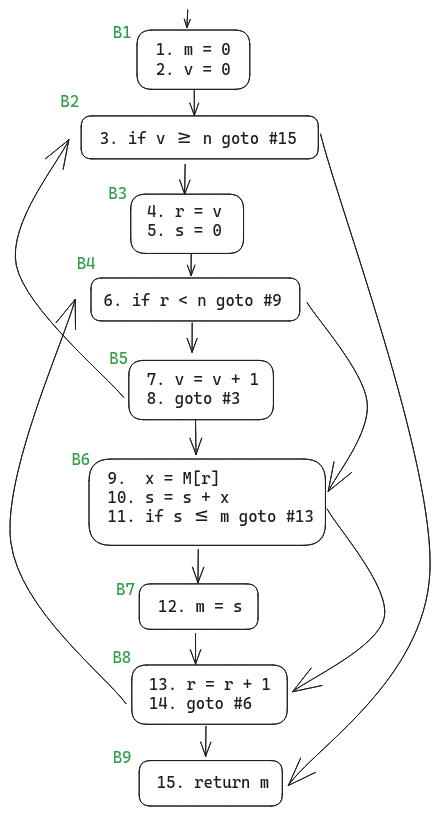
\includegraphics[width=1\textwidth]{hw4-cfg2.png}
    \end{figure}

    \section*{Question 3}

    \subsection*{3a}
    \begin{center}
        \begin{tabular}{ | c | l | l | l | l | }
            \hline
            block   & use       & def   & out           & in            \\
            \hline
            9       & m         &       &               & m             \\
            \hline
            8       & r         & r     & r,n,s,x,m,v   & r,n,s,x,m,v   \\
            \hline
            7       & s         & m     & r,n,s,x,m,v   & r,n,s,x,v         \\
            \hline
            6       & r,s,x,m   & x,s   & r,n,s,x,m,v   & r,n,s,x,m,v       \\
            \hline
            5       & v         & v     & r,s,x,m,v,n   & r,s,x,m,v,n   \\
            \hline
            4       & r,n       &       & r,s,x,m,v,n   & r,s,x,m,v,n   \\
            \hline
            3       & v         & r,s   & r,n,s,x,m,v   & v,n,x,m           \\
            \hline
            2       & v,n       &       & v,n,x,m       & v,n,x,m         \\
            \hline
            1       &           & m,v   & v,n,x,m       & n,x             \\
            \hline
        \end{tabular}
    \end{center}

    \subsection*{3b}
    Variables $n$ and $x$ are uninitialized because we see that these 2 variables are live on entry to block 1 which is at the beginning of the program. This means that these variables are used before they are defined or initialized.

    \section*{Question 4}

    \begin{center}
        \begin{tabular}{ c c c }
            \hline
            block   & dom       & idom \\
            \hline
            0       & 0         &       \\
            1       & 1,0       & 0      \\
            2       & 2,0       & 0     \\
            3       & 3,2,0     & 2     \\
            4       & 4,2,0     & 2     \\
            5       & 5,2,0     & 2     \\
            6       & 6,0       & 0     \\
            \hline
        \end{tabular}
    \end{center}

    \begin{figure}[H]
        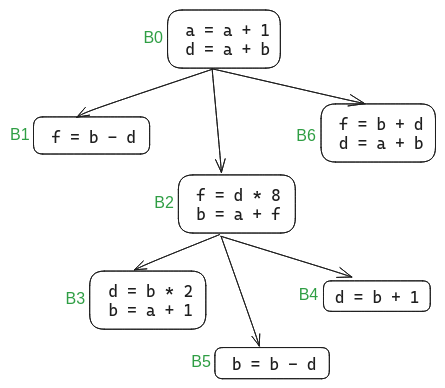
\includegraphics[width=1\textwidth]{hw4-dom4.png}
    \end{figure}

    \begin{center}
        \begin{tabular}{ c c c }
            \hline
            block   & dominance frontier        & strictly dominates \\
            \hline
            0       &                           & 1,2,3,4,5,6       \\
            1       & 6                         &       \\
            2       & 2,6                       & 3,4,5     \\
            3       & 5                         &      \\
            4       & 5                         &      \\
            5       & 2,6                       &      \\
            6       & 0                         &      \\
            \hline
        \end{tabular}
    \end{center}

    \section*{Question 5}

    \begin{figure}[H]
        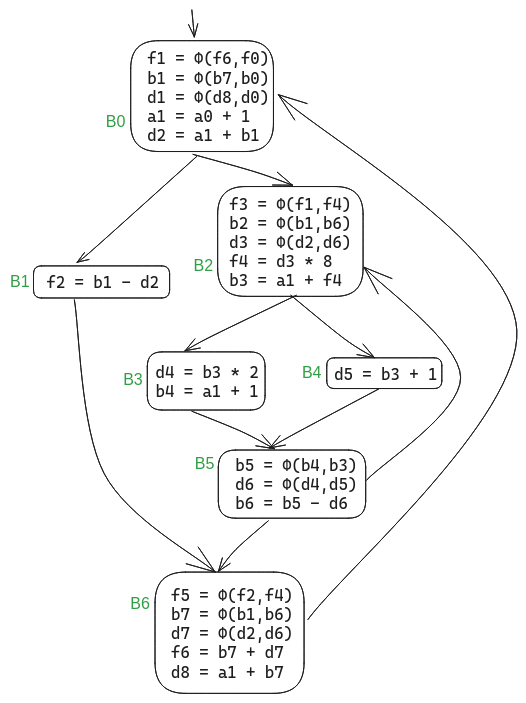
\includegraphics[width=1\textwidth]{hw4-ssa5.png}
    \end{figure}

\end{document}
